\documentclass[conference]{IEEEtran}
\usepackage[T1]{fontenc}
\usepackage{graphicx}
\usepackage{booktabs}
\usepackage{amsmath}
\usepackage{amssymb}
\usepackage{xcolor}
\usepackage[hidelinks]{hyperref}
\newcommand{\lab}[1]{\textsf{#1}}
% Generated by analysis/make_paper_assets.py -- do not edit.
\newcommand{\ExpRuns}{144}
\newcommand{\ExpRequests}{258,046}
\newcommand{\ExpCPU}{M2}
\newcommand{\ExpCores}{8}
\newcommand{\ExpRAMGiB}{16}
\newcommand{\ExpPython}{3.12.13}
\newcommand{\ExpLiboqs}{0.16.0}
\newcommand{\ExpCommit}{30e6fb9}
\newcommand{\OvhPutSmallPoneBtwo}{-14.2}
\newcommand{\OvhPutSmallPoneBone}{-0.2}
\newcommand{\OvhPutSmallRoneBone}{+0.2}
\newcommand{\LatPutSmallPone}{5.27}
\newcommand{\LatPutSmallRone}{5.29}
\newcommand{\OvhPutMidPoneBtwo}{-27.6}
\newcommand{\OvhPutMidPoneBone}{-21.2}
\newcommand{\OvhPutMidRoneBone}{-22.6}
\newcommand{\LatPutMidPone}{12.31}
\newcommand{\LatPutMidRone}{12.08}
\newcommand{\OvhGetSmallPoneBtwo}{-10.4}
\newcommand{\OvhGetSmallPoneBone}{+6.6}
\newcommand{\OvhGetSmallRoneBone}{+243.4}
\newcommand{\LatGetSmallPone}{2.62}
\newcommand{\LatGetSmallRone}{8.45}
\newcommand{\OvhGetMidPoneBtwo}{+1.0}
\newcommand{\OvhGetMidPoneBone}{+3.0}
\newcommand{\OvhGetMidRoneBone}{+90.9}
\newcommand{\LatGetMidPone}{8.04}
\newcommand{\LatGetMidRone}{14.90}
\newcommand{\ClientShareKESmall}{33}
\newcommand{\ClientShareSerSmall}{45}
\newcommand{\ClientShareAeadSmall}{5}
\newcommand{\KEShareSmall}{2.1}
\newcommand{\StorageShareSmall}{93.5}
\newcommand{\ClientShareKELarge}{3}
\newcommand{\ClientShareSerLarge}{3}
\newcommand{\ClientShareAeadLarge}{92}
\newcommand{\KEShareLarge}{0.1}
\newcommand{\StorageShareLarge}{97.0}
\newcommand{\MicroPoneEnc}{17.4}
\newcommand{\MicroPoneDec}{20.1}
\newcommand{\MicroRoneEnc}{91.9}
\newcommand{\MicroRoneDec}{6,126}
\newcommand{\MicroBtwoEnc}{250.1}
\newcommand{\MicroBtwoDec}{165.6}
\newcommand{\MicroPtwoEnc}{271.8}
\newcommand{\MicroRoneOverPone}{305}
\newcommand{\MicroHKDF}{4.8}
\newcommand{\MicroAESGiBs}{7.1}
\newcommand{\NOnePutReductionHundred}{8.5}
\newcommand{\NOnePutReductionTen}{4.2}
\newcommand{\NOneGetReductionHundred}{9.9}
\newcommand{\NOneGetReductionTen}{4.7}
\newcommand{\MemSmallest}{3}
\newcommand{\MemLargest}{51}
\newcommand{\MemLargestSize}{500}
\newcommand{\MemSmallestSize}{1}

% Generated by analysis/revision_assets.py -- do not edit.
\newcommand{\RevRuns}{1{,}165}
\newcommand{\RevRequests}{78.3}
\newcommand{\RevFailures}{0}
\newcommand{\RevInvalid}{0}
\newcommand{\RevSettleMedian}{3.0}
\newcommand{\RevLinkGbit}{12.4}
\newcommand{\RevRtt}{0.32}
\newcommand{\RevDiskRead}{1{,}970}
\newcommand{\RevDiskWrite}{850}
\newcommand{\ArmRuns}{330}
\newcommand{\ArmRequests}{19.4}
\newcommand{\ArmFailures}{0}
\newcommand{\ArmInvalid}{0}
\newcommand{\ArmSettleMedian}{3.0}
\newcommand{\ArmLinkGbit}{14.9}
\newcommand{\ArmRtt}{0.16}
\newcommand{\ArmDiskRead}{2{,}010}
\newcommand{\ArmDiskWrite}{870}
\newcommand{\RevRegion}{ap-southeast-2}
\newcommand{\RevClientCPU}{Intel Xeon Platinum 8488C}
\newcommand{\RevKernel}{7.0.0}
\newcommand{\RevCommit}{33ea9ce}
\newcommand{\ArmClientCPU}{AWS Graviton3}
\newcommand{\ArmKernel}{7.0.0}
\newcommand{\ArmCommit}{3fb4366}
\newcommand{\RevAllRuns}{1{,}495}
\newcommand{\RevAllRequests}{97.6}
\newcommand{\RevBatchERuns}{300}
\newcommand{\RevBatchEKRuns}{80}
\newcommand{\RevBatchFRuns}{380}
\newcommand{\RevBatchGRuns}{195}
\newcommand{\RevBatchHRuns}{210}
\newcommand{\RevBatchIRuns}{210}
\newcommand{\RevBatchIKRuns}{60}
\newcommand{\RevBatchIOneRuns}{60}
\newcommand{\RevPrimaryEq}{6}
\newcommand{\RevPrimaryInc}{2}
\newcommand{\RevPrimaryDiff}{0}
\newcommand{\RevPrimaryEqTwoPct}{5}
\newcommand{\RevPrimaryEqTenPct}{8}
\newcommand{\RevPrimaryNoStallSame}{8}
\newcommand{\RevPrimaryStalledPairs}{1}
\newcommand{\RevHotRatio}{0.960}
\newcommand{\RevHotDeficit}{4.0}
\newcommand{\RevHotCI}{0.959--0.962}
\newcommand{\RevNoisyRatio}{1.000}
\newcommand{\RevNoisyCI}{0.94--1.06}
\newcommand{\RevNoisySd}{11}
\newcommand{\RevKneeRatio}{1.017}
\newcommand{\RevKneeCI}{0.987--1.048}
\newcommand{\RevKneeP}{0.041}
\newcommand{\RevKneePHolm}{0.083}
\newcommand{\RevKneeSd}{8}
\newcommand{\RevLargeRatioLo}{0.998}
\newcommand{\RevLargeRatioHi}{1.001}
\newcommand{\RevXwingHotDeficit}{9.6}
\newcommand{\RevXwingMidDeficit}{4.5}
\newcommand{\RevXwingEq}{6}
\newcommand{\RevXwingNonEq}{1}
\newcommand{\RevXwingVsMlkemHotDeficit}{5.8}
\newcommand{\ArmPrimaryEq}{6}
\newcommand{\ArmPrimaryInc}{2}
\newcommand{\ArmPrimaryDiff}{0}
\newcommand{\ArmPrimaryEqTwoPct}{4}
\newcommand{\ArmPrimaryEqTenPct}{7}
\newcommand{\ArmPrimaryNoStallSame}{8}
\newcommand{\ArmPrimaryStalledPairs}{3}
\newcommand{\ArmHotRatio}{0.951}
\newcommand{\ArmHotDeficit}{4.9}
\newcommand{\ArmHotCI}{0.950--0.953}
\newcommand{\ArmNoisyRatio}{1.026}
\newcommand{\ArmNoisyCI}{0.94--1.12}
\newcommand{\ArmNoisySd}{15}
\newcommand{\ArmKneeRatio}{1.001}
\newcommand{\ArmKneeCI}{0.968--1.036}
\newcommand{\ArmKneeP}{0.013}
\newcommand{\ArmKneePHolm}{0.040}
\newcommand{\ArmKneeSd}{9}
\newcommand{\ArmLargeRatioLo}{0.992}
\newcommand{\ArmLargeRatioHi}{1.001}
\newcommand{\ArmXwingHotDeficit}{10.4}
\newcommand{\ArmXwingMidDeficit}{4.9}
\newcommand{\ArmXwingEq}{4}
\newcommand{\ArmXwingNonEq}{1}
\newcommand{\ArmXwingVsMlkemHotDeficit}{5.9}
\newcommand{\RevStudyHybridEq}{8}
\newcommand{\RevStudyHybridLo}{0.969}
\newcommand{\RevRsaGetLo}{0.42}
\newcommand{\RevRsaGetHi}{0.46}
\newcommand{\RevKeEcdhPut}{0.089}
\newcommand{\RevKeShareEcdhPut}{2.3}
\newcommand{\RevKeEcdhGet}{0.049}
\newcommand{\RevKeShareEcdhGet}{2.2}
\newcommand{\ArmKeEcdhPut}{0.109}
\newcommand{\ArmKeShareEcdhPut}{3.2}
\newcommand{\ArmKeEcdhGet}{0.068}
\newcommand{\ArmKeShareEcdhGet}{3.5}
\newcommand{\RevKeMLKEMPut}{0.045}
\newcommand{\RevKeShareMLKEMPut}{1.2}
\newcommand{\RevKeMLKEMGet}{0.047}
\newcommand{\RevKeShareMLKEMGet}{2.2}
\newcommand{\ArmKeMLKEMPut}{0.058}
\newcommand{\ArmKeShareMLKEMPut}{1.7}
\newcommand{\ArmKeMLKEMGet}{0.063}
\newcommand{\ArmKeShareMLKEMGet}{3.3}
\newcommand{\RevKeStudyHybridPut}{0.133}
\newcommand{\RevKeShareStudyHybridPut}{3.4}
\newcommand{\RevKeStudyHybridGet}{0.097}
\newcommand{\RevKeShareStudyHybridGet}{4.5}
\newcommand{\RevKeXwingPut}{0.142}
\newcommand{\RevKeShareXwingPut}{3.6}
\newcommand{\RevKeXwingGet}{0.133}
\newcommand{\RevKeShareXwingGet}{5.8}
\newcommand{\ArmKeXwingPut}{0.177}
\newcommand{\ArmKeShareXwingPut}{5.1}
\newcommand{\ArmKeXwingGet}{0.167}
\newcommand{\ArmKeShareXwingGet}{8.2}
\newcommand{\RevKeShareXwingLarge}{0.10}
\newcommand{\RevMatrixStudyHybridLo}{0.90}
\newcommand{\RevMatrixStudyHybridHi}{1.07}
\newcommand{\RevMatrixStudyHybridWithin}{15}
\newcommand{\RevMatrixXwingLo}{0.91}
\newcommand{\RevMatrixXwingHi}{1.02}
\newcommand{\RevMatrixXwingWithin}{15}
\newcommand{\RevMatrixCells}{18}
\newcommand{\RevMatrixXwingCpuHi}{21}
\newcommand{\RevHybridRssDiffMedian}{4}
\newcommand{\RevHybridRssDiffMedianPct}{0.4}
\newcommand{\RevHybridRssDiffMaxPct}{5}
\newcommand{\RevMetaEcdh}{622}
\newcommand{\RevMetaMLKEM}{2{,}034}
\newcommand{\RevMetaStudyHybrid}{2{,}085}
\newcommand{\RevMetaXwing}{2{,}074}
\newcommand{\RevMetaExtraMLKEM}{1{,}412}
\newcommand{\RevMetaExtraXwing}{1{,}452}
\newcommand{\RevMetaXwingOverMLKEM}{40}
\newcommand{\RevMetaBillionTB}{1.41}
\newcommand{\RevMetaBillionTiB}{1.28}
\newcommand{\RevMetaMillionGB}{1.41}
\newcommand{\RevMetaMillionGiB}{1.32}
\newcommand{\RevSessCpuSavingLo}{2.1}
\newcommand{\RevSessCpuSavingHi}{3.7}
\newcommand{\RevSessThroughputLo}{0.966}
\newcommand{\RevSessThroughputHi}{1.062}
\newcommand{\RevSessThroughputSig}{0}
\newcommand{\RevSessConfigs}{9}
\newcommand{\RevSessBoneCpu}{1.7}
\newcommand{\RevSessShortKem}{0.0038}
\newcommand{\RevSessShortObjects}{248}
\newcommand{\RevSessShortObjectsMax}{310}
\newcommand{\RevSessLightObjects}{94}
\newcommand{\RevSessLightKem}{0.0107}
\newcommand{\RevSessLightHundredObjects}{94}
\newcommand{\RevSessFullKem}{0.0011}
\newcommand{\RevSessHundredCpuSaving}{3.0}
\newcommand{\RevSessGetGain}{3.3}
\newcommand{\RevSessGetGainLo}{3.1}
\newcommand{\RevSessGetGainHi}{3.5}
\newcommand{\RevSessGetBone}{0.992}
\newcommand{\RevQSmallPeak}{4{,}820}
\newcommand{\RevQSmallOverload}{4{,}300}
\newcommand{\RevQSmallLastStable}{3{,}600}
\newcommand{\RevQSmallFirstUnstable}{3{,}900}
\newcommand{\RevQSmallRhoLastStable}{0.75}
\newcommand{\RevQSmallRhoFirstUnstable}{0.81}
\newcommand{\RevQSmallKneeLo}{3{,}600}
\newcommand{\RevQSmallKneeHi}{3{,}900}
\newcommand{\RevQSmallHeldOut}{3}
\newcommand{\RevQSmallMapeMmc}{16}
\newcommand{\RevQSmallKneeMmc}{4{,}300}
\newcommand{\RevQSmallMapeState}{8}
\newcommand{\RevQSmallKneeState}{4{,}190}
\newcommand{\RevQSmallMapeLoad}{8}
\newcommand{\RevQSmallKneeLoad}{4{,}070}
\newcommand{\RevQSmallServiceLight}{4.7}
\newcommand{\RevQSmallServiceOverload}{51}
\newcommand{\RevQMidPeak}{4{,}410}
\newcommand{\RevQMidOverload}{4{,}120}
\newcommand{\RevQMidLastStable}{3{,}300}
\newcommand{\RevQMidFirstUnstable}{3{,}600}
\newcommand{\RevQMidRhoLastStable}{0.75}
\newcommand{\RevQMidRhoFirstUnstable}{0.82}
\newcommand{\RevQMidKneeLo}{3{,}000}
\newcommand{\RevQMidKneeHi}{3{,}300}
\newcommand{\RevQMidHeldOut}{2}
\newcommand{\RevQMidMapeMmc}{13}
\newcommand{\RevQMidKneeMmc}{4{,}080}
\newcommand{\RevQMidMapeState}{4}
\newcommand{\RevQMidKneeState}{3{,}890}
\newcommand{\RevQMidMapeLoad}{4}
\newcommand{\RevQMidKneeLoad}{3{,}270}
\newcommand{\RevQMidServiceLight}{5.4}
\newcommand{\RevQMidServiceOverload}{59}
\newcommand{\RevProfFutexTime}{45}
\newcommand{\RevProfNamespaceTime}{35}
\newcommand{\RevProfNamespaceCalls}{65}
\newcommand{\RevProfWriteTime}{5}
\newcommand{\RevProfSyncTime}{1.1}
\newcommand{\RevProfSyncPerObject}{0.17}
\newcommand{\RevProfDirectoryPerObject}{19}
\newcommand{\RevProfStraceCycles}{14}
\newcommand{\RevProfDiskAwait}{0.20}
\newcommand{\RevProfDiskAwaitPninetyfive}{0.58}
\newcommand{\RevProfDiskUtil}{76}
\newcommand{\RevProfDiskQueue}{3.0}
\newcommand{\RevProfDiskSeconds}{292}
\newcommand{\RevProfDiskWriteMib}{283}
\newcommand{\RevProfCpuUser}{68}
\newcommand{\RevProfCpuKernel}{31}
\newcommand{\RevProfCpuKernelLocks}{6}
\newcommand{\RevProfPerfCycles}{12}
\newcommand{\RevOrderShiftMax}{1.1}
\newcommand{\RevOrderShiftMaxQuiet}{1.1}
\newcommand{\RevCvQuietMax}{2.2}
\newcommand{\RevCvNoisyLo}{4}
\newcommand{\RevCvNoisyHi}{9}
\newcommand{\RevStalls}{8}
\newcommand{\RevStallsSmallPut}{8}
\newcommand{\ArmStalls}{3}
\newcommand{\ArmStallsSmallPut}{3}
\newcommand{\RevNoisyCpuCorr}{0.91}
\newcommand{\RevNoisyRuns}{40}

% Generated by analysis/audit_assets.py -- do not edit.
\newcommand{\AudRuns}{480}
\newcommand{\AudRequests}{41.5}
\newcommand{\AudFailures}{0}
\newcommand{\AudPadRatio}{0.993}
\newcommand{\AudPadCI}{0.991--0.995}
\newcommand{\AudPadCost}{0.7}
\newcommand{\AudRestRatio}{0.967}
\newcommand{\AudRestCI}{0.965--0.969}
\newcommand{\AudRestCost}{3.3}
\newcommand{\AudJFullRatio}{0.960}
\newcommand{\AudJFullCI}{0.958--0.962}
\newcommand{\AudPadShare}{17}
\newcommand{\AudPadShareLo}{14}
\newcommand{\AudPadShareHi}{21}
\newcommand{\AudPadVerdict}{does not explain}
\newcommand{\AudPredicted}{0.956}
\newcommand{\AudPredictionErrorJ}{0.4}
\newcommand{\AudPredictionInsideJ}{outside}
\newcommand{\AudJCpuRatio}{1.047}
\newcommand{\AudPadStageGet}{6.0}
\newcommand{\AudMlkemStageGet}{5.6}
\newcommand{\AudKdfOverPadGet}{4.3}
\newcommand{\AudJRuns}{120}
\newcommand{\AudKKneeRatio}{0.994}
\newcommand{\AudKKneeCI}{0.984--1.004}
\newcommand{\AudKKneeSd}{4}
\newcommand{\AudKKneeVerdict}{equivalent}
\newcommand{\AudKSatRatio}{0.996}
\newcommand{\AudKSatCI}{0.979--1.013}
\newcommand{\AudKSatSd}{7}
\newcommand{\AudKSatVerdict}{equivalent}
\newcommand{\AudKEq}{2}
\newcommand{\AudKEqNoStall}{2}
\newcommand{\AudKRuns}{200}
\newcommand{\AudKStalls}{6}
\newcommand{\AudBindVerdict}{explains}
\newcommand{\AudLFullRatio}{0.963}
\newcommand{\AudLFullCI}{0.960--0.967}
\newcommand{\AudLFullCost}{3.7}
\newcommand{\AudPredictionErrorL}{0.7}
\newcommand{\AudPredictionInsideL}{outside}
\newcommand{\AudBindReleasedRatio}{0.999}
\newcommand{\AudBindReleasedCI}{0.997--1.002}
\newcommand{\AudBindReleasedCost}{0.1}
\newcommand{\AudBindReleasedRemoved}{99}
\newcommand{\AudBindReleasedRemovedLo}{92}
\newcommand{\AudBindReleasedRemovedHi}{105}
\newcommand{\AudBindReleasedEqTwoPct}{yes}
\newcommand{\AudBindReleasedCpuRatio}{1.007}
\newcommand{\AudBindReleasedKeOne}{0.028}
\newcommand{\AudBindHeldRatio}{1.002}
\newcommand{\AudBindHeldCI}{0.997--1.006}
\newcommand{\AudBindHeldCost}{$-$0.2}
\newcommand{\AudBindHeldRemoved}{105}
\newcommand{\AudBindHeldRemovedLo}{94}
\newcommand{\AudBindHeldRemovedHi}{115}
\newcommand{\AudBindHeldEqTwoPct}{yes}
\newcommand{\AudBindHeldCpuRatio}{0.998}
\newcommand{\AudBindHeldKeOne}{0.027}
\newcommand{\AudBindHeldOverReleased}{1.002}
\newcommand{\AudBindHeldOverReleasedCI}{0.999--1.006}
\newcommand{\AudLCpuRatio}{1.043}
\newcommand{\AudBindBindingKeOne}{0.047}
\newcommand{\AudBindEcdhKeOne}{0.050}
\newcommand{\AudLRuns}{120}
\newcommand{\AudAllocDefaultLo}{0.12}
\newcommand{\AudAllocDefaultHi}{0.38}
\newcommand{\AudAllocDefaultSpread}{3.2}
\newcommand{\AudAllocDefaultThrSpread}{10}
\newcommand{\AudAllocFixedLo}{0.29}
\newcommand{\AudAllocFixedHi}{0.32}
\newcommand{\AudAllocFixedSpread}{1.1}
\newcommand{\AudAllocFixedThrSpread}{3}
\newcommand{\AudAllocRuns}{40}
\newcommand{\AudNRuns}{90}
\newcommand{\AudNFailures}{0}
\newcommand{\AudNGo}{1.26.2}
\newcommand{\AudNOneOps}{2{,}920}
\newcommand{\AudNOneCores}{1.00}
\newcommand{\AudNOneCpuUs}{343}
\newcommand{\AudNOneSaturated}{yes}
\newcommand{\AudNOneMlkemThr}{0.905}
\newcommand{\AudNOneMlkemThrCI}{0.900--0.910}
\newcommand{\AudNOneMlkemVerdict}{deficit}
\newcommand{\AudNOneMlkemDeficit}{9.5}
\newcommand{\AudNOneMlkemCpu}{1.105}
\newcommand{\AudNOneMlkemCpuCI}{1.099--1.111}
\newcommand{\AudNOneXwingThr}{0.826}
\newcommand{\AudNOneXwingThrCI}{0.821--0.831}
\newcommand{\AudNOneXwingVerdict}{deficit}
\newcommand{\AudNOneXwingDeficit}{17.4}
\newcommand{\AudNOneXwingCpu}{1.211}
\newcommand{\AudNOneXwingCpuCI}{1.203--1.218}
\newcommand{\AudNMidOps}{10{,}300}
\newcommand{\AudNMidCores}{9.75}
\newcommand{\AudNMidCpuUs}{947}
\newcommand{\AudNMidSaturated}{no}
\newcommand{\AudNMidMlkemThr}{0.943}
\newcommand{\AudNMidMlkemThrCI}{0.929--0.958}
\newcommand{\AudNMidMlkemVerdict}{deficit}
\newcommand{\AudNMidMlkemDeficit}{5.7}
\newcommand{\AudNMidMlkemCpu}{1.072}
\newcommand{\AudNMidMlkemCpuCI}{1.051--1.093}
\newcommand{\AudNMidXwingThr}{0.923}
\newcommand{\AudNMidXwingThrCI}{0.906--0.940}
\newcommand{\AudNMidXwingVerdict}{deficit}
\newcommand{\AudNMidXwingDeficit}{7.7}
\newcommand{\AudNMidXwingCpu}{1.117}
\newcommand{\AudNMidXwingCpuCI}{1.090--1.144}
\newcommand{\AudNHotOps}{14{,}580}
\newcommand{\AudNHotCores}{11.50}
\newcommand{\AudNHotCpuUs}{789}
\newcommand{\AudNHotSaturated}{no}
\newcommand{\AudNHotMlkemThr}{0.996}
\newcommand{\AudNHotMlkemThrCI}{0.994--0.999}
\newcommand{\AudNHotMlkemVerdict}{no deficit}
\newcommand{\AudNHotMlkemDeficit}{0.4}
\newcommand{\AudNHotMlkemCpu}{1.091}
\newcommand{\AudNHotMlkemCpuCI}{1.054--1.129}
\newcommand{\AudNHotXwingThr}{0.989}
\newcommand{\AudNHotXwingThrCI}{0.986--0.992}
\newcommand{\AudNHotXwingVerdict}{no deficit}
\newcommand{\AudNHotXwingDeficit}{1.1}
\newcommand{\AudNHotXwingCpu}{1.157}
\newcommand{\AudNHotXwingCpuCI}{1.123--1.191}
\newcommand{\AudNOneMlkemCpuDelta}{36}
\newcommand{\AudNOneXwingCpuDelta}{72}
\newcommand{\AudNMicroMlkem}{50.6}
\newcommand{\AudNMicroEcdh}{33.4}
\newcommand{\AudNMicroXwing}{85.1}
\newcommand{\AudNMicroMlkemExtra}{17}
\newcommand{\AudNMicroXwingExtra}{52}


\begin{document}
\title{Supplementary Material: Open-Loop Capacity of the Store\\[2pt]
\large for ``Benchmarking Post-Quantum Key Encapsulation in S3-Compatible Object Storage under Client Concurrency''}
\author{}
\maketitle

\section{Open-Loop Capacity of the Store}\label{sec:queue}
This supplement characterizes the store, not post-quantum cryptography. It is included to check that the key-establishment mode does not move the point at which response time degrades. All numbers are generated by the same pipeline as those of the main paper; experiment labels are those of its mapping table (\lab{Open-Loop} is batch H of the artifact).

\subsection{Queueing Models}
An M/M/c queue has Poisson arrivals at rate $\lambda$, $c$ servers and exponential service times
with mean $S$~\cite{harchol2013}. With $a=\lambda S$ the mean response time is
$W=S+C(c,a)\,S/(c-a)$, where $C$ is the Erlang~C probability of waiting. Its service time does
not depend on load. A \emph{state-dependent} birth--death queue lets the total service rate
$\mu(n)$ depend on the number $n$ of requests in the system; its stationary distribution is
$p_n\propto\prod_{k\le n}\lambda/\mu(k)$ and its mean response time follows from Little's law.


\subsection{Pre-Registered Queueing Protocol}\label{sec:qprotocol}
The 12 open-loop rates are sorted; the 1st, 3rd, \ldots{} are training points and the 2nd, 4th,
\ldots{} are held out. Models may use training points and the closed-loop runs, and are scored by
mean absolute percentage error (MAPE) on the held-out rates at which the system was stable. A
rate is stable if every run delivers at least 97\,\% of the offered rate with a mean queue wait
below 10\,ms; response times of unstable runs grow with run length and are lower bounds.


\subsection{Results}
This subsection describes the store, not post-quantum cryptography, and we include it for one
reason: to check that the choice of mode does not move the point of degradation. That closed-loop
measurements overstate what an open arrival stream can sustain is established
\cite{schroeder2006}; what we add is where the transition lies for this store.

\textbf{Two thresholds.} We distinguish the \emph{knee}, the interval of offered load in which
mean response time first exceeds twice its light-load value, from the \emph{stability boundary},
between the highest rate at which every run kept up and the lowest at which one did not. Under
Poisson arrivals of ML-KEM PUTs (\lab{Open-Loop}), with $\rho$ the offered rate over the peak closed-loop
throughput of the same experiment (\RevQSmallPeak{} and \RevQMidPeak{} requests/s): at 1\,KiB the
knee and the stability boundary coincide, between \RevQSmallKneeLo{} and \RevQSmallKneeHi{}
requests/s ($\rho=\RevQSmallRhoKneeLo$--\RevQSmallRhoKneeHi); at 64\,KiB the knee lies between
\RevQMidKneeLo{} and \RevQMidKneeHi{} requests/s ($\rho=\RevQMidRhoKneeLo$--\RevQMidRhoKneeHi)
and the stability boundary one step higher, between \RevQMidLastStable{} and
\RevQMidFirstUnstable{} ($\rho=\RevQMidRhoLastStable$--\RevQMidRhoFirstUnstable). The
confirmatory campaign measured ML-KEM only; the exploratory campaign found the knee in the same
place for the symmetric-only mode B1 and for P1, which is our evidence that the mode does not
move it.

\textbf{Models.} We compare three models (Fig.~\ref{fig:queuerev}, Table~\ref{tab:queue}).
(a)~M/M/$c$ with the light-load service time $S_0$, capacity $\mu$ from the two most overloaded
training rates and $c=\mathrm{round}(\mu S_0)$. (b)~A state-dependent queue whose service rate
$\mu(n)$ is the closed-loop throughput measured with $n$ workers, interpolated linearly; it uses
no open-loop data at all. (c)~A load-dependent fit
$W(\rho)=S_0\,[1+a\rho^{b}/(1-\rho)]$ with $\rho=\lambda/\mu$, whose two parameters are fitted to
the stable training rates.

\begin{figure}[t]
\centering
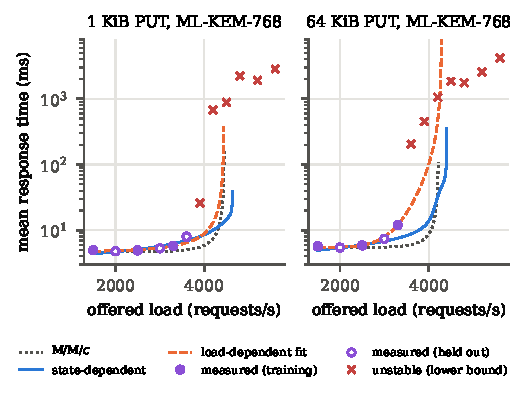
\includegraphics[width=\columnwidth]{generated/fig-queue-rev.pdf}
\caption{Open-loop mean response time of ML-KEM PUT against offered load (\lab{Open-Loop}; log scale), with three models. Filled: training rates; hollow: held-out rates; crosses: unstable rates (lower bounds).}
\label{fig:queuerev}
\end{figure}

\begin{table}[t]
\caption{Queueing models for ML-KEM PUT (requests/s). Stable/unstable: the stability boundary, i.e.\ highest stable and lowest unstable offered rate. Observed knee: interval in which mean response time first exceeds twice its light-load value; predicted knee: the rate at which each model does.}
\label{tab:queue}
\centering\footnotesize
\setlength{\tabcolsep}{2.5pt}
\resizebox{\columnwidth}{!}{% Generated by analysis/revision_assets.py -- do not edit.
\begin{tabular}{lrcc|ccc|ccc}
\toprule
 & & & & \multicolumn{3}{c|}{Held-out error (MAPE)} & \multicolumn{3}{c}{Predicted knee (req/s)} \\
Size & Peak & Stable/unstable & Observed knee & M/M/$c$ & State & Load & M/M/$c$ & State & Load \\
\midrule
1\,KiB & 4{,}820 & 3{,}600/3{,}900 & 3{,}600--3{,}900 & 16\% & 8\% & 8\% & 4{,}300 & 4{,}190 & 4{,}070 \\
64\,KiB & 4{,}410 & 3{,}300/3{,}600 & 3{,}000--3{,}300 & 13\% & 4\% & 4\% & 4{,}080 & 3{,}890 & 3{,}270 \\
\bottomrule
\end{tabular}
}
\end{table}

On the stable held-out rates (only \RevQSmallHeldOut{} at 1\,KiB and \RevQMidHeldOut{} at
64\,KiB), M/M/$c$ has a MAPE of \RevQSmallMapeMmc\,\% and \RevQMidMapeMmc\,\%; the
state-dependent model \RevQSmallMapeState\,\% and \RevQMidMapeState\,\%; the load-dependent fit
\RevQSmallMapeLoad\,\% and \RevQMidMapeLoad\,\%. The two alternatives are close to each other
but not identical. Both roughly halve the error because they let service time
rise with load, which M/M/$c$ cannot: the mean service time of a 1\,KiB PUT grows from
\RevQSmallServiceLight\,ms at the lightest rate to about \RevQSmallServiceOverload\,ms in
overload.

\textbf{The knee is still predicted too late.} M/M/$c$ places the knee at \RevQSmallKneeMmc{} and
\RevQMidKneeMmc{} requests/s and the state-dependent model at \RevQSmallKneeState{} and
\RevQMidKneeState, both above the observed intervals. The fitted model matches at 64\,KiB
(\RevQMidKneeLoad) and is late at 1\,KiB (\RevQSmallKneeLoad). The reason is visible in the data:
the state-dependent model assumes the store can sustain its mean closed-loop throughput, but in
overload the open-loop runs achieved only \RevQSmallOverload{} and \RevQMidOverload{} requests/s,
below the closed-loop peaks, and closed-loop throughput itself varies by several percent between
runs at high concurrency. A system whose capacity fluctuates becomes unstable when the offered
rate reaches the lower part of that range, not its mean. With only \RevQSmallHeldOut{} and
\RevQMidHeldOut{} stable held-out points per size, these error figures are indicative rather than
precise, and the fitted model is a description of this configuration, not a general law.

\textbf{Summary.} For this store, response time doubles at
\RevQMidRhoKneeLo--\RevQSmallRhoKneeHi{} of peak closed-loop throughput and runs become unstable
at \RevQSmallRhoLastStable--\RevQMidRhoFirstUnstable. Letting service time depend on load halves
the prediction error of M/M/c below the knee, on very few held-out points; no model we tested
predicts the knee from closed-loop capacity.



\bibliographystyle{IEEEtran}
\bibliography{references}
\end{document}
